\begin{figure}[!htb] 
        \centering
        \begin{subfigure}[b]{1.8in}
                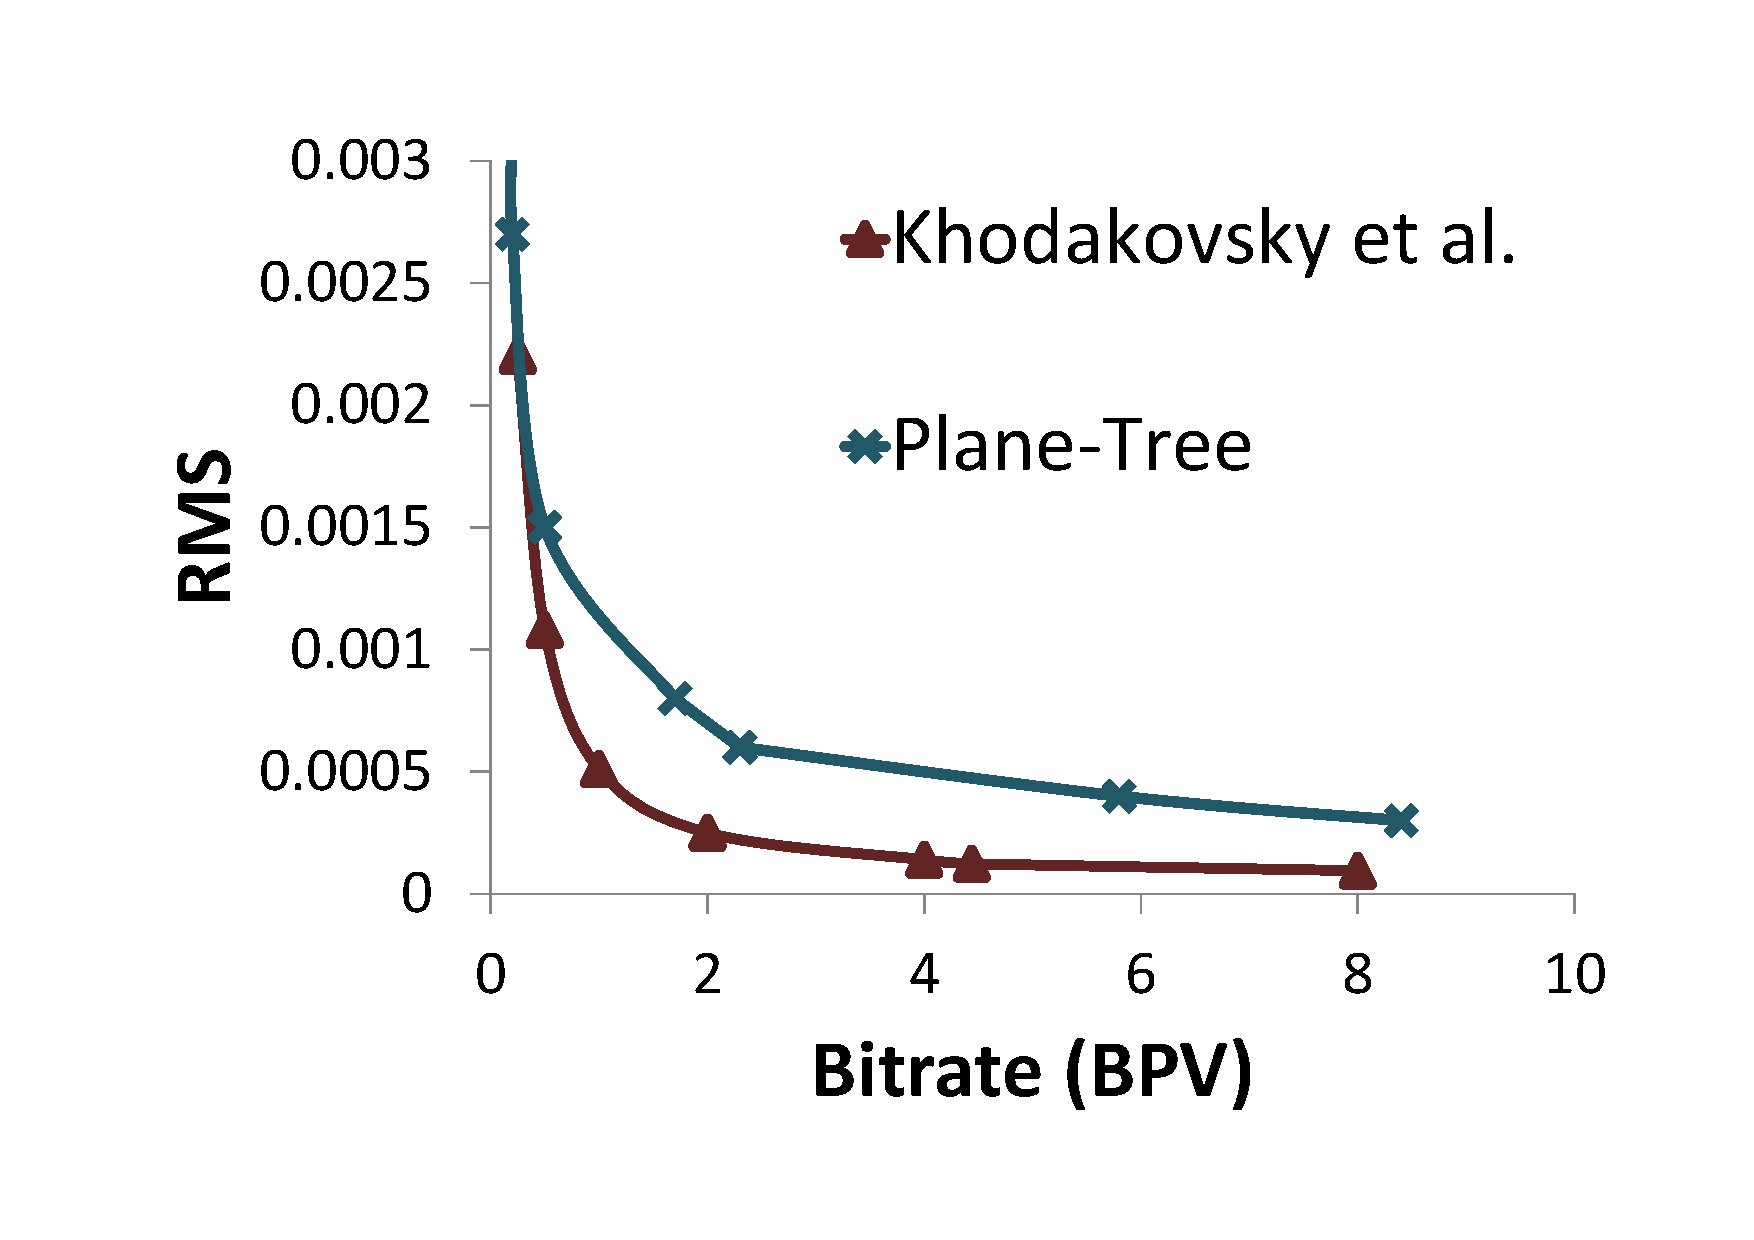
\includegraphics[width=1.8in]{images/results/compression/bunnysota}
                \caption{Bunny Model}
                \label{fig:SA_BUNNY}
        \end{subfigure}%
        \begin{subfigure}[b]{1.8in}
                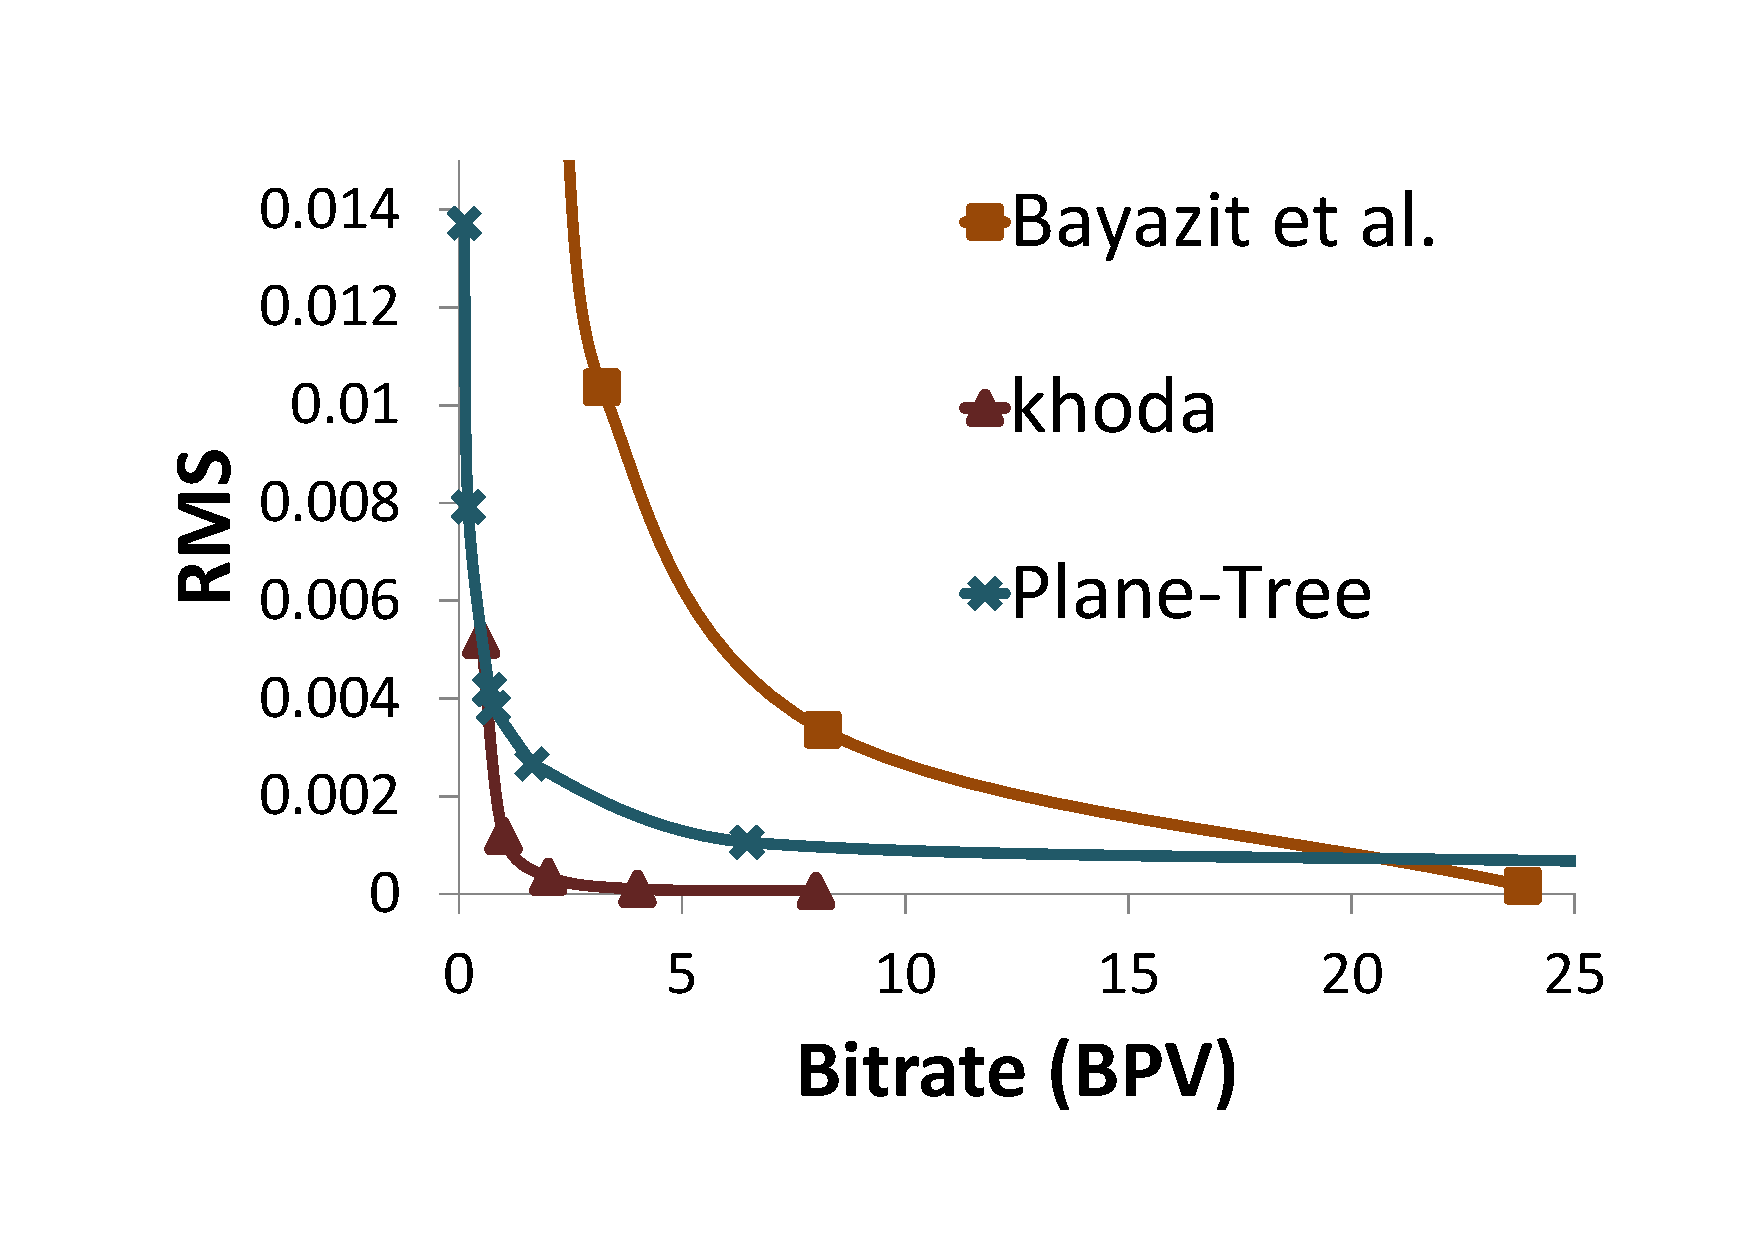
\includegraphics[width=1.8in]{images/results/compression/fandisksota}
                \caption{Fandisk Model}
                \label{fig:SA_FANDISK}
        \end{subfigure}
        
        \begin{subfigure}[b]{1.8in}
                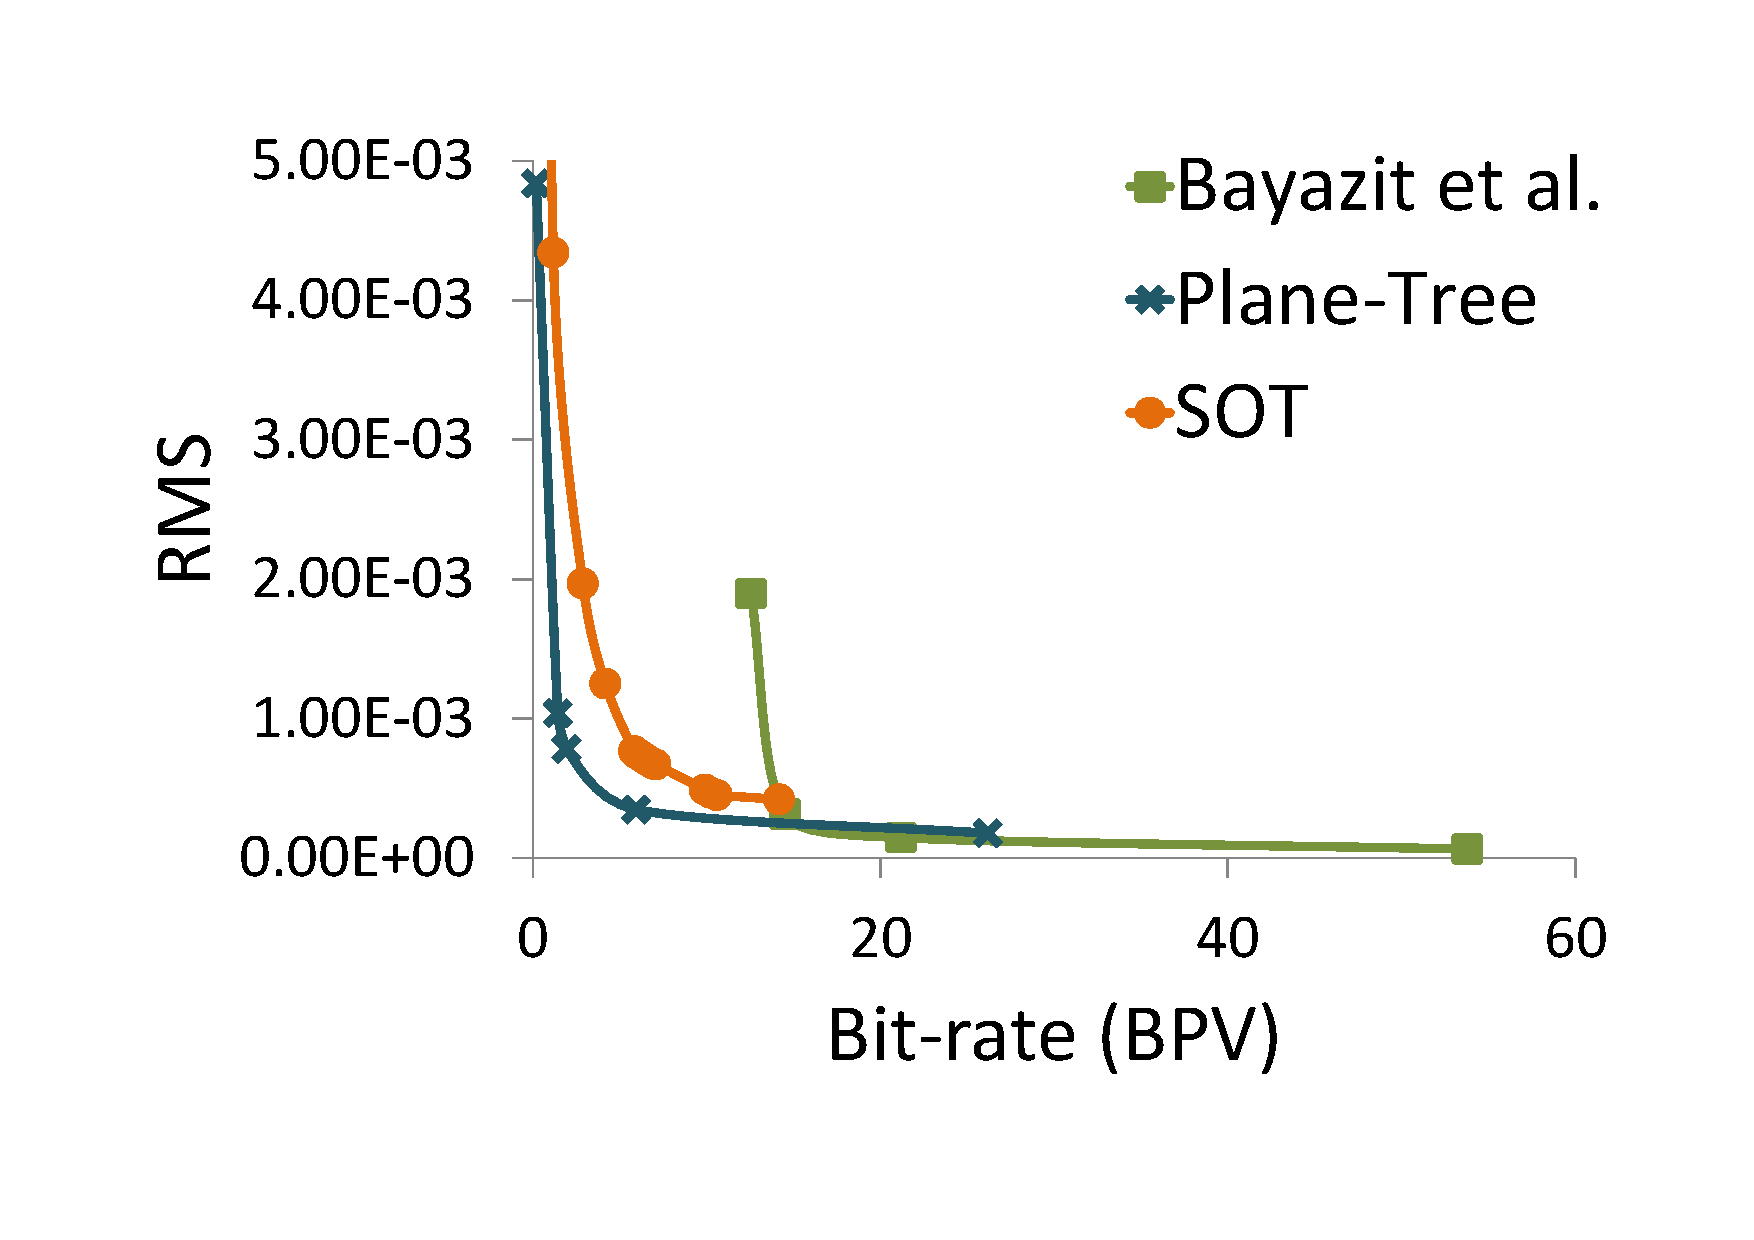
\includegraphics[width=1.8in]{images/results/compression/horsesota}
                \caption{Horse Model}
                \label{fig:SA_HORSE}
        \end{subfigure}%
        \begin{subfigure}[b]{1.8in}
                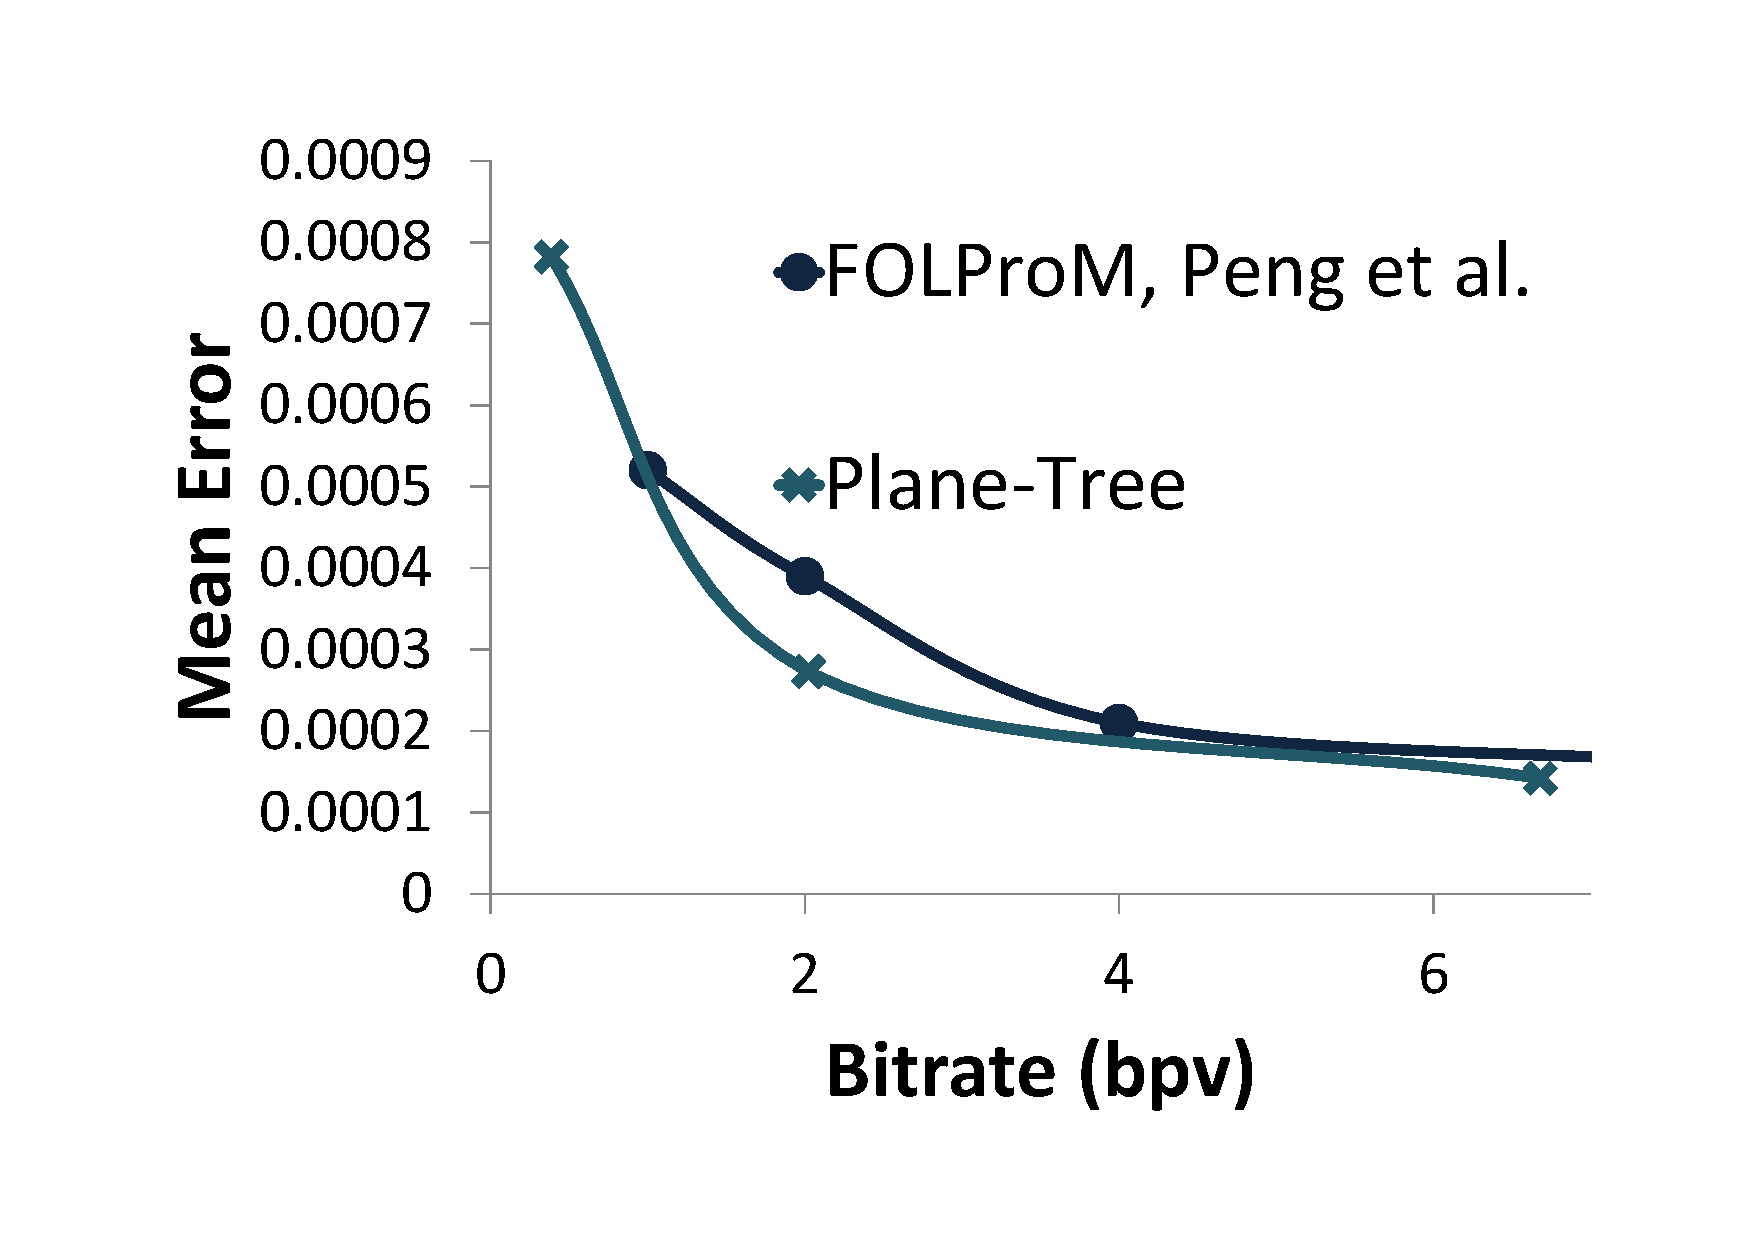
\includegraphics[width=1.8in]{images/results/compression/rabbitsota}
                \caption{Rabbit Model}
                \label{fig:SA_RABBIT}
        \end{subfigure}
       \caption{Rate-Distortion graphs comparing the Plane-Tree to different state of the art codecs.}
       \label{fig:SOTAEXPS}
\end{figure}

In figures \ref{fig:SA_BUNNY}, \ref{fig:SA_FANDISK} and \ref{fig:SA_HORSE} we compare the Plane-Tree with the state of the art transform methods by Bayazit et al \cite{Bayazit103DMesh} and Khodakovsky et al \cite{Khodakovsky00Progressive}. \\

Experiment results comparing the Plane-Tree compression system proposed in this work with the transform-based method by Khodakovsky et al are shown in figure \ref{fig:SA_BUNNY}. This Rate-Distortion graph shows that the Plane-Tree has similar performance with the method by Khodakovsky et al. At low bit-rates the Plane-Tree is highly competitive the with performance matching Khodakovsky's. The competitiveness extends to higher bit-rates as well for the bunny model. \\

Figure \ref{fig:SA_FANDISK} shows comparisons between the Plane-Tree as well as methods by Khodakovsky et al and Bayazit et al. Here, both the Plane-Tree and the method by Khodakovsky et al perform similarly as in the bunny model experiment (figure \ref{fig:SA_BUNNY}). The Plane-Tree stays competitive with that state of the art method, and improves upon the compression performance in comparison to the spectral compression method by Bayazit et al. It can be seen that at low to mid bit-rates, the Plane-Tree method compressed the Fandisk model at a higher level of quality for a given bit-rate. \\

The Plane-Tree was also compared with Bayazit et al using another model, the horse model. Figure \ref{fig:SA_HORSE} shows the result of this experiment. The Plane-Tree method outperforms the transform based method of Bayazit et al whilst decreasing coding complexity compared to the complicated transform method. Overall, in this experiment, the proposed Plane-Tree method remains competitive at higher bitrates, and it outperforms the method by Bayazit et al at lower bitrates. \\

Finally the Plane-Tree is compared with the state of the art low-bitrate compression system FOLProM presented by Peng et al \cite{Peng10Feature}. Unlike the other experiments, the mean-error metric is used in this comparison, as the results presented by Peng et al used this metric. It can be seen that at low-bitrates (below 2 bits per vertex), the Plane-Tree method outperforms this state of the art low-bitrate compression system. \\


In conclusion, these experiments show that the Plane-Tree is extremely competitive with the state of the art compression systems at high bit-rates. At lower bit-rates it improves upon the results by these methods. This algorithm is also powerful in that it may be used to compress 3D volumetric data as well as point-cloud and mesh data. This makes it an interesting candidate for 3D reconstruction compression no matter the format output by a given 3D reconstruction method. \\